\begin{figure}
  \vskip-1ex
  \centering
  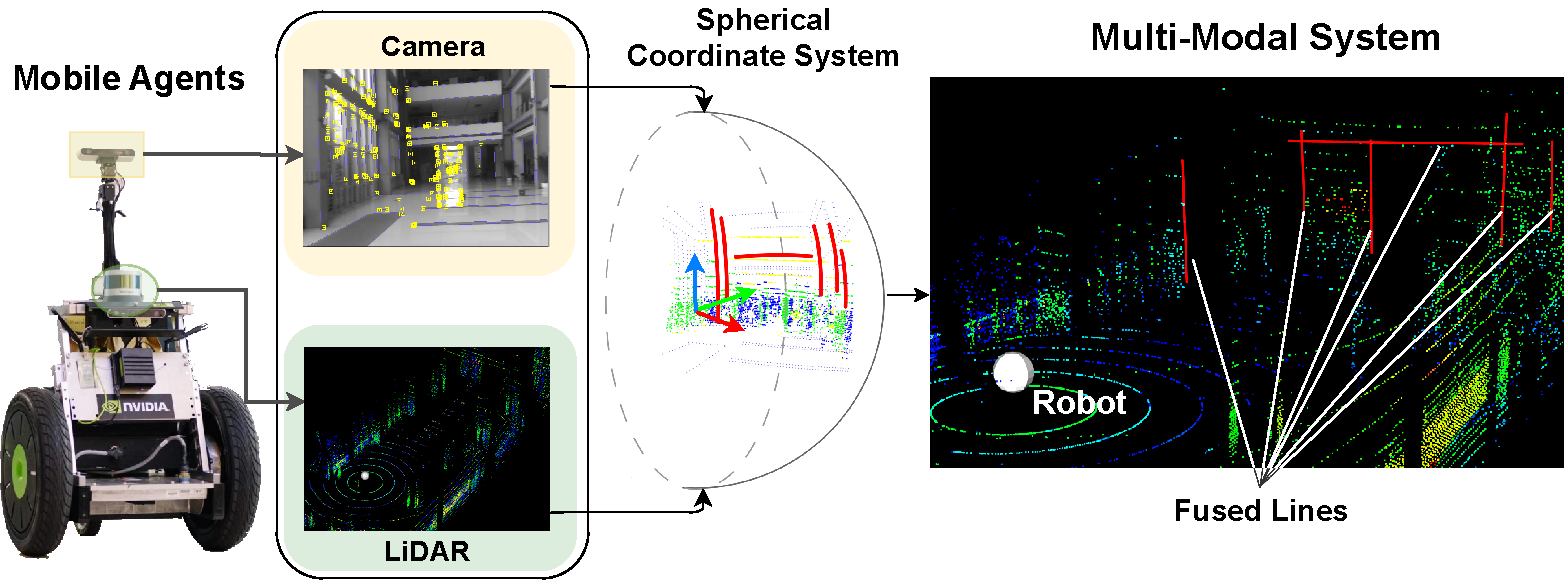
\includegraphics[width=0.5\textwidth]{images/robot2.pdf}
  \vskip-2ex
  \caption{Our method projects the geometric features (extracted from the sensor camera and LiDAR data) onto the fusion frame (the spherical coordinate system). Through a series of optimizations, a more accurate trajectory and map are obtained with the reconstructed line.} 
  \label{fig:overview_intro}
  \vskip -3ex
\end{figure}
%
In the field of mobile robots and autonomous navigation agents, there has been a notable increase of interest among different studies \cite{pandey2017mobile, zhu2021deep, patle2019review}. 
They are employed for a variety of purposes, including independent living for the elderly~\cite{cortes2007assistive, sasaki2009human}, guiding and assisting shoppers in large retail spaces~\cite{orciuoli2015agent, qu2021outline}, and facilitating delivery services in outdoor industrial or commercial areas~\cite{abbenseth2017cloud, lopez2017predictive}. When a robot enters a new scene or encounters an environment with updated details, it carefully plans actions to explore unknown or uncertain areas. The goal is to gather valuable information about the new terrain and improve the accuracy of its reconstructed map. Thereby, the robot utilizes the measurements provided by its sensors to reconstruct the map and perform localization through SLAM. 

Tracking failure in challenging environments has hindered the widespread adoption of mobile robots. While visual SLAM \cite{forster2014svo, mur2015orb, mur2017orb} offers superior motion estimation, it tends to fail in extreme lighting conditions and outdoor environments. Similarly, LiDAR SLAM~\cite{deschaud2018imls, shan2018lego, zhang2014loam} is highly reliable for tracking motion in large-scale scenes but faces challenges in degraded cases. Traditional SLAM methods rely heavily on a single source, which may be prone to failure in adverse scenarios or due to equipment issues. In recent years, significant approaches~\cite{chou2021efficient, shan2021lvi, zhu2021camvox} have been developed to integrate measurements from multiple sensors to overcome the limitations of mono-sensor algorithms. However, some SLAM systems~\cite{chou2021efficient} combine camera, IMU, and LiDAR to recalibrate the extrinsic parameters which can be quite computationally expensive. Therefore, our research focuses on the development of a camera-LiDAR framework. The primary goal of this framework is to minimize sensor costs for mobile agents while conserving computational resources. Moreover, it aims to provide highly accurate mapping and localization in a variety of scenarios.

%
In practical situations, devices often oscillate when in motion. This leads to less accurate extrinsic calibration between the camera and the LiDAR. The fusion performance~\cite{graeter2018limo}, which relies solely on the association of feature points, is highly susceptible to the misalignment error caused by this oscillation. Consequently, inaccurate depth estimates are obtained, compromising the overall accuracy of the system.
Other SLAM methods~\cite{fang2020visual, lee2021plf, pumarola2017pl} that depend on geometric features prove that lines are more reliable and stable. Therefore, our work is exclusively concentrated on geometric-level fusion to combine the monocular camera and LiDAR sensors.

In this paper, we propose a multi-modal SLAM system that tightly integrates parallel monocular visual SLAM and LiDAR SLAM subsystems. This design ensures that if one subsystem fails, the other subsystem continues to operate, providing a more robust system for robot navigation. Moreover, we utilize more stable linear and planar features to minimize the impact of inaccurate extrinsic calibration. In Figure~\ref{fig:overview_intro}, each subsystem utilizes perceptual data from the mobile robot's sensors (a camera and a LiDAR sensor) to extract geometric features. We align the features from both subsystems in terms of temporality, spatiality, and dimensionality through a unified reference fusion frame. After fusion, the reconstructed features contribute as new landmarks to the initial pose estimation in the visual subsystem. They are utilized as additional optimization parameters in the back end, where the endpoint and direction are used to constrain the visual odometry. In the LiDAR subsystem, the direction of the geometric features is adjusted by the detected line from the visual system, reducing the probability of outliers during registration.

We evaluate our approach on the M2DGR dataset \cite{yin2021m2dgr}, which consists of various indoor and outdoor environments commonly encountered in mobile robot applications. By comparing with our visual baselines Structure PLP-SLAM~\cite{shu2022structure}, LiDAR baseline MULLS~\cite{pan2021mulls}, and multi-modal algorithms LVI-SAM~\cite{shan2021lvi} and ORB-SLAM3~\cite{campos2021orb}, our SLAM method achieves superior accuracy and robustness in various challenging environments. It is particularly suitable for low-cost mobile robots in various applications.

To summarize, we present the following contributions:

\begin{compactitem}
\item We build a fusion framework -- a spherical coordinate system -- to maintain spatial and temporal consistency. This framework integrates the geometric features from the visual subsystem and the LiDAR subsystem.

\item In the LiDAR subsystem, we optimize the linear directions to improve registration efficiency and accuracy, while increasing the probability of optimized points in its local map.

\item We reconstruct more lines for pose estimation in the visual subsystem. In the back end of the visual subsystem, we propose a new optimization term, \textit{i.e.}, line direction term, and more fusion lines as optimization parameters to constrain the trajectory.

\end{compactitem}